
%Copyright (C) 2016 by Krishneel@JSK Lab, The University of Tokyo

\documentclass{standalone}
\begin{document}

\subsection{Hardware}
For task 3, we used two types of UAVs; the $Hawk$ which is similar to the one used in task 1 and a transformable UAV called the $Snake$.
Since all the UAVs uses the same custom built control board, the central control hardware components almost the same as those used for task 1, except that we designed an additional PCB board for controlling the Electronic-Magnet. We equipped 5 Electromagnets on the UAV and build the attachment with tactile sensors. The electromagnet control board is connected to the central control unit through CAN bus.

The $Snake$ has a snake-like structure with for propeller units connected by actuated joints. It is capable of changing its configuration during flight, and allows grasping of objects by enclosing its body around the object. 

\subsection{Software}
As with other tasks the software are build using ROS and some functionalities are shared with task 1. Point Cloud and OpenCV libraries are used for visual perception. % target detection and motion planning are different.

\subsection{General Approach}
%The software system is based on ROS(Robot Operation System). We write our algorithm to the every single node and communicate with each node. 
\subsubsection{Overall Strategy}
We divide the task into three states: Search, Pick, and Place. The UAVs are always in one of these three states and the states automatically transition into the next one if the certain conditions are satisfied as illustrated in Fig. \ref{t3}A. In the "Search" state, the drone will traverse to the center of the arena and randomly generate a search end-point, the treasure detector will run while the drone is searching. Once the object is detected and locked, a pick motion will be generated in the "Pick" state, the UAV will turn on the electromagnet and approach the treasure (for the $Hawk$) or enclose its body around the treasure (for the $Snake$). The state transition is signalled by the trigger of the tactile sensor. Once the electromagnet of the $Hawk$ has caught the treasure or the body of the $Snake$ has enclosed the treasure, the UAV transition into the next state. In the "Place" state, the UAV will fly directly to the placing zone and find the box to place the treasure. After releasing the treasure into the place box, the UAV re-enters the "Search" state and loops until the task is completed.

 \begin{figure}%[hb]
    \begin{center}
      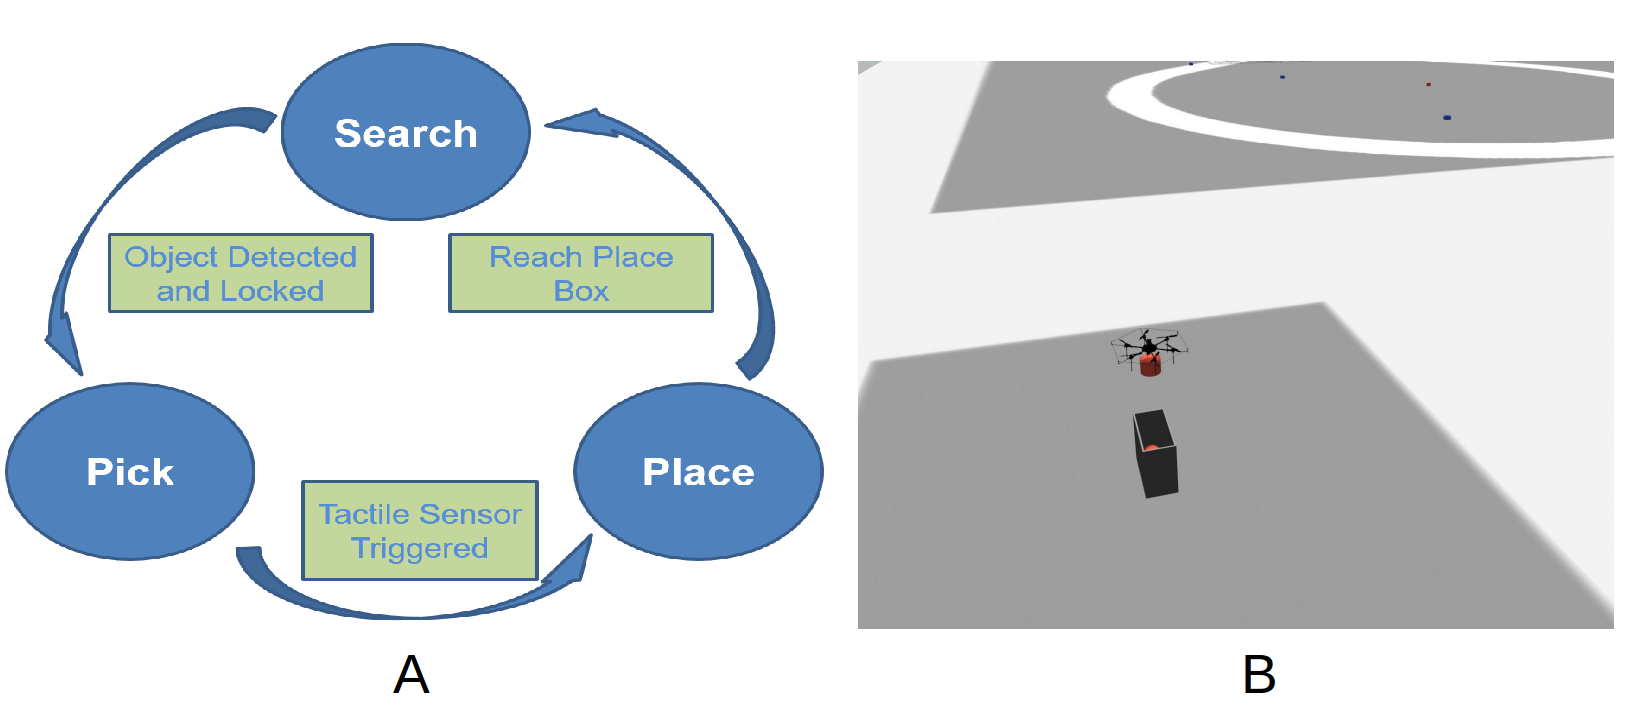
\includegraphics[keepaspectratio=true, width=1\linewidth, height=0.30\textheight]{img//task3.png}
    \end{center}
    \caption{Task 3 Demonstration}
    \label{t3}
  \end{figure}



\subsubsection{Treasure Detection}
As the treasures have distinct color features, we first used a simple detection method to detect the treasures. 
The inputs are 3D points $p_i$ from the Stereo sensor and the RGB image projection onto the ground by the projection matrix computed using the known camera parameters. %We first apply 
HSI color filter is applied to obtain the 3D point candidates of the treasures from the point cloud data. Next we apply Euclidean clustering to the filtered point cloud $P_{hsi}$. Euclidean clustering technique can organize points into clusters with respect to distance features in 3D space. For $\forall p_i, p_j \in P_{hsi}$, clusters $O_i = \{p_i \in P_i\}$ and $O_j = \{p_j \in P_j\}$ are obtained by:
\begin{equation}\label{eq3-1}
min||p_i - p_j|| \geq d_{threhold} 
\end{equation}
After we obtained all the clusters, we apply a simple tracker to every cluster center and as we continue to detect the same cluster over time space, the weight of the tracker is increased to boost the confidence of tracking. For clusters that are not always detected the confidence are slowly decreased and removed from the treasure candidates vector. The UAV will lock on to the cluster candidate when the weight is large enough and switch into the "Pick" mode to approach the treasure.

\subsection{Results Achieved to Date}
We performed full automatic simulation in gazebo environment as shown in Fig.\ref{t3}B. To fully simulate the real scene, we add noise and outliers to the detection. In simulation, the UAV takes almost 70 $seconds$ to detect, pick and place a single object. 
% we believe we can do that better. 
With the real robots, we tested tele-operation control, and both the $Hawk$ and the $Snake$ were able to grasp the treasure and pick and place it into a specified box. 

\subsection{Future Plans}
In our next steps, we will use three UAVs in coordination to complete the task which will not only decrease the time but also can be used to transport larger treasures which a single UAV might not be able to lift. We will also be carrying out more experiments on the real robots to test the detection and motion planning algorithm that have been verified in simulation.


\end{document}
